\documentclass{report}
\usepackage[utf8]{inputenc}
\usepackage[T1]{fontenc}
\usepackage{hyperref}
\usepackage{geometry}
\usepackage{listings}
\usepackage{xcolor}
\usepackage{textcomp}
\usepackage{standalone}
\usepackage{import}
\usepackage{graphicx}
\usepackage{float}

\geometry{a4paper, margin=1in}

% Define the flag so sub-files know not to print title pages
\newcommand{\maindoc}{true}

\definecolor{codegreen}{rgb}{0,0.6,0}
\definecolor{codegray}{rgb}{0.5,0.5,0.5}
\definecolor{codepurple}{rgb}{0.58,0,0.82}
\definecolor{backcolour}{rgb}{0.95,0.95,0.92}

\lstdefinestyle{mystyle}{
    backgroundcolor=\color{backcolour},   
    commentstyle=\color{codegreen},
    keywordstyle=\color{magenta},
    numberstyle=\tiny\color{codegray},
    stringstyle=\color{codepurple},
    basicstyle=\ttfamily\footnotesize,
    breakatwhitespace=false,         
    breaklines=true,                 
    captionpos=b,                    
    keepspaces=true,                 
    numbers=left,                    
    numbersep=5pt,                  
    showspaces=false,                
    showstringspaces=false,
    showtabs=false,                  
    tabsize=2,
    upquote=true,
    extendedchars=true
}

\lstdefinelanguage{TypeScript}{
  keywords={typeof, new, true, false, catch, function, return, null, catch, switch, var, if, in, while, do, else, case, break},
  keywordstyle=\color{blue}\bfseries,
  ndkeywords={class, export, boolean, throw, implements, import, this},
  ndkeywordstyle=\color{darkgray}\bfseries,
  identifierstyle=\color{black},
  sensitive=false,
  comment=[l]{//},
  morecomment=[s]{/*}{*/},
  commentstyle=\color{purple}\ttfamily,
  stringstyle=\color{red}\ttfamily,
  morestring=[b]',
  morestring=[b]"
}

\lstset{style=mystyle}

\title{Educational Movie Database Software Manual \\[0.5cm] "CineLearn" (Cinematic Learning)}
\author{324827328, 213713522 \\[2cm] \includegraphics[width=0.7\textwidth]{images/sql-meme.jpeg}}
\date{}

\begin{document}

\maketitle

\tableofcontents

\chapter{Client Application}
\documentclass{article}
\usepackage[utf8]{inputenc}
\usepackage[T1]{fontenc}
\usepackage{hyperref}
\usepackage{geometry}
\usepackage{listings}
\usepackage{xcolor}
\usepackage{textcomp}

\geometry{a4paper, margin=1in}

\definecolor{codegreen}{rgb}{0,0.6,0}
\definecolor{codegray}{rgb}{0.5,0.5,0.5}
\definecolor{codepurple}{rgb}{0.58,0,0.82}
\definecolor{backcolour}{rgb}{0.95,0.95,0.92}

\lstdefinestyle{mystyle}{
    backgroundcolor=\color{backcolour},   
    commentstyle=\color{codegreen},
    keywordstyle=\color{magenta},
    numberstyle=\tiny\color{codegray},
    stringstyle=\color{codepurple},
    basicstyle=\ttfamily\footnotesize,
    breakatwhitespace=false,         
    breaklines=true,                 
    captionpos=b,                    
    keepspaces=true,                 
    numbers=left,                    
    numbersep=5pt,                  
    showspaces=false,                
    showstringspaces=false,
    showtabs=false,                  
    tabsize=2,
    upquote=true,
    extendedchars=true
}

\lstdefinelanguage{TypeScript}{
  keywords={typeof, new, true, false, catch, function, return, null, catch, switch, var, if, in, while, do, else, case, break},
  keywordstyle=\color{blue}\bfseries,
  ndkeywords={class, export, boolean, throw, implements, import, this},
  ndkeywordstyle=\color{darkgray}\bfseries,
  identifierstyle=\color{black},
  sensitive=false,
  comment=[l]{//},
  morecomment=[s]{/*}{*/},
  commentstyle=\color{purple}\ttfamily,
  stringstyle=\color{red}\ttfamily,
  morestring=[b]',
  morestring=[b]"
}

\lstset{style=mystyle}

\title{Client Software Manual}
\author{324827328, 213713522}
\date{}

\begin{document}

\ifdefined\maindoc
\else
  \maketitle
  \tableofcontents
  \newpage
\fi

\section{Introduction}
The development of the client-side application using Angular focused on creating a responsive and interactive user interface.

\section{Technologies}
Choosing the right tools was the first major decision we faced. We chose technologies based on two reasons, the first one is how much we can learn from it. For example, we really wanted to try out the new Angular Signals API, which we werent familiar with. The second reason is more technical:

\subsection{TypeScript}
We utilized TypeScript to leverage static typing in our development process. This provided type safety and facilitated refactoring, helping to identify potential errors across the codebase during compilation rather than at runtime.

\subsection{Angular}
We chose Angular because we wanted a framework that included everything out of the box. Unlike other libraries where you have to hunt for a router or a state management solution, Angular gave us a complete toolkit. We were particularly excited to use the new \textbf{Signals} feature. It allowed us to manage the complexity of our application state—like keeping the search results in sync with the selected genres—without writing complex boilerplate code.

\subsection{Chart.js}
For the analytics dashboard, we needed a library that could handle heavy lifting. We tried a few options, but Chart.js stood out because of its performance with the canvas element. When you're rendering multiple bar charts showing thousands of data points (like budget vs. revenue for flops), you need something that won't freeze the browser.

\subsection{RxJS}
RxJS was employed to manage asynchronous operations. As the application relies heavily on backend communication, Observables were used to handle complex data flows, such as coordinating concurrent API requests (using \texttt{forkJoin}) and managing search input streams (using \texttt{switchMap}).

\section{Components}
We broke the application down into three main areas, each addressing a specific user need.

\subsection{The Home Page (HomeComponent)}
The Home component (\texttt{client/src/app/components/home/home.ts}) serves as the primary interface for content discovery. A key technical requirement was the implementation of a responsive filtering system that updates results based on both text input and genre selection.

Instead of writing a complex chain of event listeners, we used a reactive approach. We created a "computed" signal that listens to both the search bar and the genre checkboxes. Whenever either changes, it automatically re-runs the filter logic.

\begin{lstlisting}[language=TypeScript, caption={Our reactive filtering solution}]
filteredMovies = computed(() => {
  const query = this.searchQuery();
  const selectedGenres = this.selectedGenres();
  
  // This re-runs automatically whenever query or selectedGenres changes
  return this.movies().filter(movie => {
    const matchesSearch = movie.title.toLowerCase().startsWith(query.toLowerCase());
    const matchesGenre = selectedGenres.size === 0 ||
      movie.genres.some(genre => selectedGenres.has(genre));
    return matchesSearch && matchesGenre;
  });
});
\end{lstlisting}

\subsection{Movie Details (MovieDetailComponent)}
The Detail view (\texttt{client/src/app/components/movie-detail/movie-detail.ts}) displays comprehensive movie metadata including cast, crew, and financial statistics.

A user identification mechanism was implemented to allow ratings without requiring account registration.

\subsubsection{Shadow Identity}
When a user visits for the first time, we check their local storage. If they don't have an ID, we generate a random string and save it. This acts as their "shadow identity," allowing us to track their votes across sessions.

\begin{lstlisting}[language=TypeScript, caption={Creating a persistent user identity}]
private getUserId(): string {
  let userId = localStorage.getItem('cinelearn_user_id');
  if (!userId) {
    // Generate a sufficiently random ID
    userId = 'user_' + Math.random().toString(36).substring(2, 15) + 
             Math.random().toString(36).substring(2, 15);
    localStorage.setItem('cinelearn_user_id', userId);
  }
  return userId;
}
\end{lstlisting}

\subsubsection{Optimistic UI}
To enhance perceived performance, we implemented an optimistic UI for the voting system. The interface updates the vote count and user rating immediately upon submission, verifying the operation with the server in the background.

\begin{lstlisting}[language=TypeScript, caption={Handling the rating submission}]
submitRating(): void {
  const movie = this.movie();
  const rating = Number(this.userRating());
  
  if (movie && rating >= 0 && rating <= 10) {
    this.movieService.rateMovie(movie.id, rating, this.userId)
      .pipe(takeUntilDestroyed(this.destroyRef))
      .subscribe({
        next: (response) => {
          this.message.set('Rating submitted successfully!');
          // We save it locally so the user sees their own vote next time
          localStorage.setItem(`rating_${movie.id}_${this.userId}`, rating.toString());
          
          // And we update the global stats with the fresh data from the server
          const updated = { 
             ...movie, 
             vote_average: response.vote_average, 
             vote_count: response.vote_count 
          };
          this.movie.set(updated);
        },
        error: (e) => {
          this.message.set('Error submitting rating.');
        }
      });
  } 
}
\end{lstlisting}

\subsection{Analytics Dashboard (AnalyticsComponent)}
The Analytics component (\texttt{client/src/app/components/analytics/analytics.ts}) visualizes statistical data derived from the movie database.

\subsubsection{Performance Challenges}
Initial testing revealed latency issues during data loading, as the application awaited all data sources before rendering.

We solved this by decoupling the data loading. Instead of one giant request, we made each chart independent. We used Angular's `toSignal` to transform each HTTP request into a signal that updates its specific chart whenever it arrives. This means the "Top Actors" chart might pop in first, followed by "Genres", keeping the user engaged while the heavier data loads.

\begin{lstlisting}[language=TypeScript, caption={Decoupled data loading}]
// This doesn't block the rest of the application
readonly popularGenres = toSignal(
  this.movieService.getPopularGenres(),
  { initialValue: [] as any[] }
);

// This runs in parallel
readonly topActors = toSignal(
  this.movieService.getTopActors(),
  { initialValue: [] as any[] }
);
\end{lstlisting}

\section{Caveats \& Usage Notes}

\subsection{The "Soft Session" Trade-off}
You might notice there isn't a login screen. We consciously chose a "soft session" approach. The user ID is stored in the browser's Local Storage. This lowers the barrier to entry—anyone can just start rating movies immediately. The trade-off is that if you clear your cache, you become a new user. For this kind of public workshop application, we felt this was the right call.

\subsection{One Vote Rule}
To prevent spam, we enforced a rule: one vote per movie per user. However, we didn't want to lock users in. If you change your mind, you can rate again, and your new vote overwrites the old one. We handle this logic on the backend, but the frontend reflects it by loading your previous rating whenever you revisit a movie page.

\end{document}


\chapter{Backend API}
\documentclass{article}
\usepackage[utf8]{inputenc}
\usepackage[T1]{fontenc}
\usepackage{hyperref}
\usepackage{geometry}
\usepackage{listings}
\usepackage{xcolor}
\usepackage{textcomp}

\geometry{a4paper, margin=1in}

\definecolor{codegreen}{rgb}{0,0.6,0}
\definecolor{codegray}{rgb}{0.5,0.5,0.5}
\definecolor{codepurple}{rgb}{0.58,0,0.82}
\definecolor{backcolour}{rgb}{0.95,0.95,0.92}

\lstdefinestyle{mystyle}{
    backgroundcolor=\color{backcolour},   
    commentstyle=\color{codegreen},
    keywordstyle=\color{magenta},
    numberstyle=\tiny\color{codegray},
    stringstyle=\color{codepurple},
    basicstyle=\ttfamily\footnotesize,
    breakatwhitespace=false,         
    breaklines=true,                 
    captionpos=b,                    
    keepspaces=true,                 
    numbers=left,                    
    numbersep=5pt,                  
    showspaces=false,                
    showstringspaces=false,
    showtabs=false,                  
    tabsize=4,
    upquote=true,
    extendedchars=true
}

\lstset{style=mystyle}

\title{Backend Software Manual}
\author{324827328, 213713522}
\date{}

\begin{document}

\ifdefined\maindoc
\else
  \maketitle
  \tableofcontents
  \newpage
\fi

\section{Introduction}
The backend for the Movie Database was designed with a focus on performance, reliability, and modularity. We adopted a layered architecture to ensure clear separation of concerns: Routers manage HTTP requests, the Repository layer abstracts database interactions, and the application logic connects these components.

\section{Technologies}
We selected a technology stack that prioritizes development efficiency and system stability.

\subsection{Python}
Python serves as the core language for our development. Its concise syntax allows for efficient expression of complex logic. Whether for data migration scripts or defining API endpoints, Python's readability facilitates maintenance and debugging.

\subsection{FastAPI}
FastAPI was chosen for its high performance and modern features, representing a significant improvement over older frameworks.
\begin{enumerate}
    \item \textbf{Performance}: Utilizing modern Python features like \texttt{async/await}, it offers high throughput comparable to lower-level languages.
    \item \textbf{Automatic Documentation}: The automatic generation of Swagger UI documentation facilitates efficient endpoint testing and verification.
    \item \textbf{Data Validation}: Integration with Pydantic ensures rigorous data validation, rejecting invalid requests automatically.
\end{enumerate}

\subsection{Uvicorn}
Uvicorn serves as the ASGI server for the application, enabling the handling of concurrent connections efficiently without blocking.

\subsection{MySQL Connector}
The \texttt{mysql-connector} library provides robust database connectivity. We encapsulated this within a \texttt{Repository} class to manage connection pooling and execution automatically.

\subsection{Pandas}
Pandas was utilized to efficienty import and process large CSV datasets. It allowed for in-memory data cleaning and transformation before migration to the SQL database.

\subsection{Python-Dotenv}
\texttt{python-dotenv} is used to manage environment variables, ensuring that sensitive credentials are kept secure in a local \texttt{.env} file and excluding them from version control.

\section{Core Infrastructure}

\subsection{The Entry Point (\texttt{main.py})}
This file initializes the application. We configured the CORS middleware to allow requests from the Angular frontend, which operates on a different port (4200).

\begin{lstlisting}[language=Python, caption={CORS Configuration}]
app.add_middleware(
    CORSMiddleware,
    allow_origins=["http://localhost:4200"], # Allow our Angular app
    allow_credentials=True,
    allow_methods=["*"],
    allow_headers=["*"],
)
\end{lstlisting}

\subsection{The Data Access Layer}
To maintain a clean codebase, we implemented a generic `Repository` class in `app/repository.py`. This class wraps database interactions, managing connection pools and executing queries safely.

\begin{lstlisting}[language=Python, caption={Database execution wrapper}]
@staticmethod
def fetch_all(query: str, params: Optional[tuple] = None) -> List[Dict[str, Any]]:
    conn = get_db_connection()
    # We use dictionary=True so we get real column names, not just tuples
    cursor = conn.cursor(dictionary=True)
    try:
        cursor.execute(query, params or ())
        return cursor.fetchall()
    finally:
        # Always clean up, even if the query fails
        cursor.close()
        conn.close()
\end{lstlisting}

\section{How It Works: API Modules}

\subsection{Movies Router (\texttt{routers/movies.py})}
A key challenge here was the "N+1 Problem". A naive approach would query the `movies` table once, and then run additional queries for each movie to fetch related data.

We addressed this by using "Bulk Fetching". We query the movies to obtain IDs, then execute optimized queries to fetch all related genres, cast, and crew data in bulk, mapping them in memory.

\begin{lstlisting}[language=Python, caption={Aggregation in memory}]
# 1. Get the movie IDs
movie_ids = [m['id'] for m in movies]

# 2. Get all related data in bulk
genres_data = Repository.fetch_all(f"SELECT ... WHERE movie_id IN ({placeholders})", movie_ids)

# 3. Map them in memory
genres_by_movie = defaultdict(list)
for g in genres_data:
    genres_by_movie[g['movie_id']].append(g['genre_name'])

# 4. Attach to movie objects
for movie in movies:
    movie['genres'] = genres_by_movie[movie['id']]
\end{lstlisting}

\subsubsection{The Rating Transaction}
We perform ratings transactionally to ensure data consistency. We insert the rating and update the movie's average score within the same operation.

\begin{lstlisting}[language=Python, caption={Transactional update}]
# Step 1: Insert the user's rating
Repository.execute("INSERT INTO ratings ... ON DUPLICATE KEY UPDATE...", (...))

# Step 2: Update the movie's cached average immediately
Repository.execute("UPDATE movies SET vote_average = %s ...", (...))
\end{lstlisting}

\subsection{Analytics Router (\texttt{routers/analytics.py})}
These endpoints perform complex aggregation queries. For example, to identify "Flops", we calculate the difference between budget and revenue at the database level.

\begin{lstlisting}[language=Python, caption={Analytics query example}]
@router.get("/analytics/flops")
def flops():
    # We let the database engine do the subtraction and sorting
    query = """
        SELECT title, budget, revenue, (budget - revenue) as loss
        FROM movies
        WHERE budget > 1000000 AND revenue < budget AND revenue > 0
        ORDER BY loss DESC
        LIMIT 10
    """
    return Repository.fetch_all(query)
\end{lstlisting}

\end{document}


\chapter{Database Schema}
\documentclass{article}
\usepackage[utf8]{inputenc}
\usepackage[T1]{fontenc}
\usepackage{hyperref}
\usepackage{geometry}
\usepackage{listings}
\usepackage{xcolor}
\usepackage{textcomp}

\geometry{a4paper, margin=1in}

\definecolor{codegreen}{rgb}{0,0.6,0}
\definecolor{codegray}{rgb}{0.5,0.5,0.5}
\definecolor{codepurple}{rgb}{0.58,0,0.82}
\definecolor{backcolour}{rgb}{0.95,0.95,0.92}

\lstdefinestyle{mystyle}{
    backgroundcolor=\color{backcolour},   
    commentstyle=\color{codegreen},
    keywordstyle=\color{magenta},
    numberstyle=\tiny\color{codegray},
    stringstyle=\color{codepurple},
    basicstyle=\ttfamily\footnotesize,
    breakatwhitespace=false,         
    breaklines=true,                 
    captionpos=b,                    
    keepspaces=true,                 
    numbers=left,                    
    numbersep=5pt,                  
    showspaces=false,                
    showstringspaces=false,
    showtabs=false,                  
    tabsize=2,
    upquote=true,
    extendedchars=true
}

\lstset{style=mystyle}

\title{Database Schema Manual}
\author{324827328, 213713522}
\date{}

\begin{document}

\ifdefined\maindoc
\else
  \maketitle
  \tableofcontents
  \newpage
\fi

\section{Introduction}
The database design was a critical component of the project, establishing a foundation for API performance and application integrity. We aimed for a normalized schema to minimize redundancy while maintaining the flexibility required for analytical queries. MySQL 8.4 was selected for its reliability and support for referential integrity.

\section{The Core Entities}

\subsection{Movies}
The \texttt{movies} table is the central entity of the database. We explicitly included \texttt{vote\_average} and \texttt{vote\_count} fields in this table.

This denormalization strategy was chosen to optimize read performance. Instead of calculating averages from the \texttt{ratings} table for every query, we maintain these aggregated values transactionally.

\begin{lstlisting}[language=SQL, caption=The heart of the system]
CREATE TABLE IF NOT EXISTS movies (
    id INT PRIMARY KEY,
    title VARCHAR(500) NOT NULL,
    -- We keep the aggregated stats right here for speed
    vote_average FLOAT,
    vote_count INT,
    -- ... other metadata
    budget BIGINT,
    revenue BIGINT,
    status VARCHAR(50)
);
\end{lstlisting}

\subsection{People}
We unified actors, directors, and writers into a single \texttt{people} table. This approach avoids data duplication for individuals who fulfill multiple roles (e.g., both acting and directing).

\begin{lstlisting}[language=SQL, caption=A unified People table]
CREATE TABLE IF NOT EXISTS people (
    id INT PRIMARY KEY,
    name VARCHAR(255) NOT NULL,
    gender INT, 
    profile_path VARCHAR(255)
);
\end{lstlisting}

\section{Connecting the Dots: Relationships}
The database relational structure defines the connections between entities.

\subsection{The Cast \& Crew}
Connecting \texttt{movies} to \texttt{people} required more than a simple link. We needed to know \textit{what role} they played.
For the \textbf{Cast}, we stored the \texttt{character\_name} and an \texttt{order\_index}. The index is crucial because it allows the frontend to validly display the "Top Billed" actors first, rather than a random alphabetical list.
For the \textbf{Crew}, it's about the \texttt{job} and \texttt{department}. This granular detail allows us to answer interesting questions like "Which directors also acted in their own movies?"

\begin{lstlisting}[language=SQL, caption=Linking People to Movies]
CREATE TABLE IF NOT EXISTS cast_members (
    credit_id VARCHAR(255) PRIMARY KEY,
    movie_id INT,
    person_id INT,
    character_name VARCHAR(500),
    order_index INT,
    FOREIGN KEY (movie_id) REFERENCES movies(id),
    FOREIGN KEY (person_id) REFERENCES people(id)
);
\end{lstlisting}

\subsection{Categorization (Genres, Keywords)}
We handled categories like Genres and Keywords as Many-to-Many relationships. This means a movie can be both "Action" and "Comedy". We separated the names into their own lookup tables (\texttt{genres}, \texttt{keywords}) and used junction tables (\texttt{movie\_genres}) to link them. This makes searching for "All Action movies" incredibly fast because it's just a simple index lookup.

\section{User Interaction}

\subsection{Ratings}
We built the \texttt{ratings} table to capture the user voice. We decided to use a string-based \texttt{user\_id} to align with our "Soft Session" strategy on the client. This table grows the fastest, so we kept it lightweight: just who, what, what score, and when.

\begin{lstlisting}[language=SQL, caption=Capturing user votes]
CREATE TABLE IF NOT EXISTS ratings (
    id INT AUTO_INCREMENT PRIMARY KEY,
    movie_id INT,
    user_id VARCHAR(255) NOT NULL,
    rating FLOAT,
    timestamp DATETIME DEFAULT CURRENT_TIMESTAMP,
    FOREIGN KEY (movie_id) REFERENCES movies(id)
);
\end{lstlisting}

\section{Binary Storage}

\subsection{Storing Images in the DB}
We opted to store movie posters directly in the database using the \texttt{LONGBLOB} data type.
While external storage (like S3) is a common pattern, storing images within the database ensures the dataset is self-contained. This simplifies backup and deployment procedures by keeping the entire application state in a single location.

\begin{lstlisting}[language=SQL, caption=Self-contained image storage]
CREATE TABLE IF NOT EXISTS movie_posters (
    movie_id INT PRIMARY KEY,
    image LONGBLOB,
    FOREIGN KEY (movie_id) REFERENCES movies(id)
);
\end{lstlisting}

\end{document}


\ifdefined\maindoc
\else
  \documentclass{report}
  \usepackage[utf8]{inputenc}
  \usepackage{graphicx}
  \title{Bonus: Exceptional UI Design}
  \author{324827328, 213713522}
  \date{}
  \begin{document}
  \maketitle
\fi

\chapter{Bonus: Exceptional UI Design}

\section{Philosophy}
The design objective was to create a modern, user-friendly interface comparable to commercial streaming platforms, moving beyond standard administrative layouts.

\section{Visual Identity}
\subsection{Glassmorphism}
We utilized a modern "Glassmorphism" aesthetic. By using semi-transparent backgrounds with background blur filters, we created a sense of depth and hierarchy. The movie cards are visually distinguished from the background, separating the foreground content from the ambient background to enhance user focus. We specifically chose this style, because apple recently updated all there devices to this style, and we wanted to learn how to build it ourselves.

\subsection{Micro-Interactions}
Subtle hover effects were implemented on interactive elements. Buttons elevate slightly, and movie posters illuminate upon interaction. These micro-interactions provide tactile feedback, enhancing the responsiveness of the application.

\subsection{Color Palette}
We selected a curated palette of deep midnight blues for the background and vibrant accents for actions, replacing standard primary colors. This dark mode-first approach reduces eye strain and highlights the movie artwork.

\section{Evolution}
The journey to this design wasn't immediate. We started with a functional but stark layout and iterated towards the polished version we have today.

\begin{figure}[h]
    \centering
    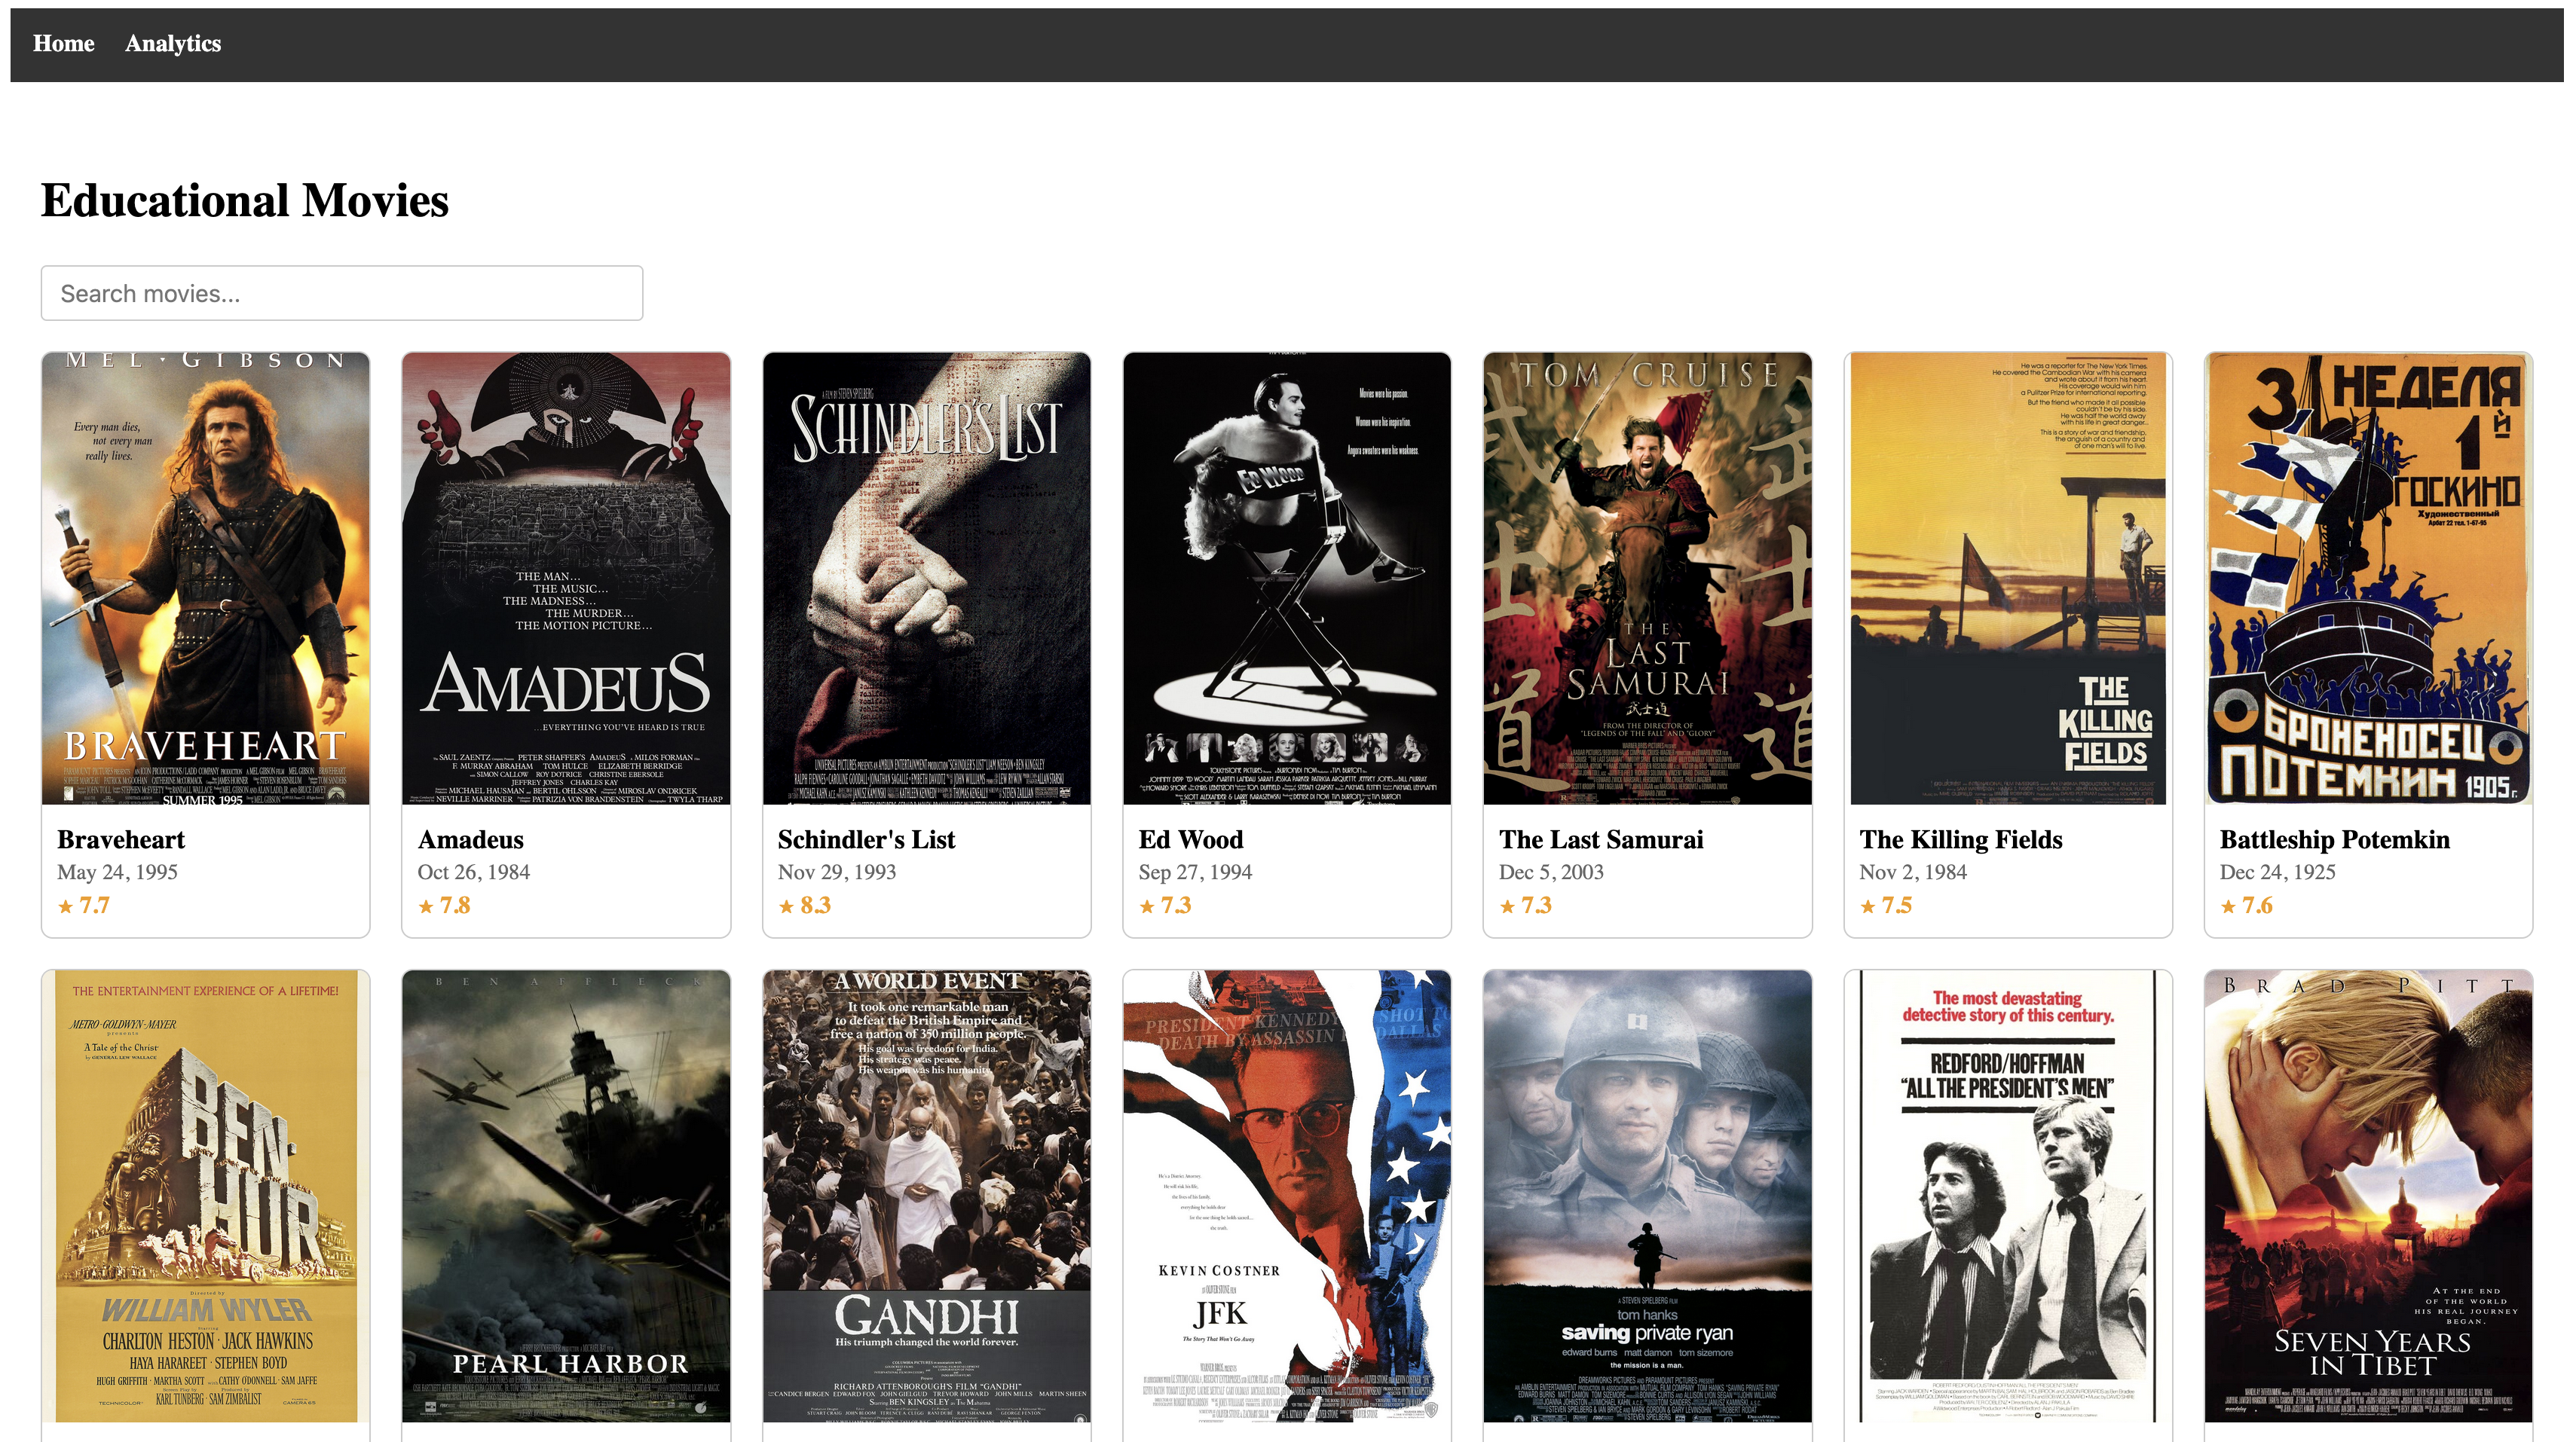
\includegraphics[width=0.9\textwidth]{../ui/images/old_ui.png}
    \caption{The initial functional prototype.}
    \label{fig:old_ui}
\end{figure}

\begin{figure}[h]
    \centering
    \includegraphics[width=0.9\textwidth]{../ui/images/new_ui.png}
    \caption{The final design with rich imagery and dark mode.}
    \label{fig:new_ui}
\end{figure}

\ifdefined\maindoc
\else
  \end{document}
\fi


\end{document}
